\chapter{Media Item Deduplication}
\label{cha:media-item-deduplication}

% the code below specifies where the figures are stored
\ifpdf
    \graphicspath{{6_media_item_deduplication/figures/PNG/}{6_media_item_deduplication/figures/PDF/}{6_media_item_deduplication/figures/}}
\else
    \graphicspath{{6_media_item_deduplication/figures/EPS/}{6_media_item_deduplication/figures/}}
\fi

\section{Introduction}

In the previous \autoref{cha:media-item-extraction},
we have motivated the need for media item deduplication.
By clustering media items, we get a~higher-level view on
a~media item cluster's overall performance on different networks.
As detailed in \autoref{sec:definition}, media items can be
photos or videos.
WordNet~\cite{fellbaum1998wordnet,miller1995wordnet} defines
the term \emph{duplicate} as
\textit{``a copy that corresponds to an original exactly''}.
The corresponding verb \emph{to duplicate} is defined as to
\textit{``make a~duplicate or duplicates of''}.
The derived term \emph{deduplication} in consequence refers to
the act of eliminating duplicate or redundant information.

\subsection{Definition of Camera Shot Boundary Detection}

In video production and filmmaking, a~shot is a~series of frames
that runs for an uninterrupted period of time.
Shots are always filmed with a~single camera and can be of any duration. 
Camera shot boundary detection is a~field of research of video processing.

\subsection{Definition of Social Media Item}

We define a~social media item as either a~photo (image) or video
that was \emph{publicly} shared or published
on at least one social network.
In the following, we will use the shorter term media item
rather than the full term.

\subsection{Definition of Exact Duplicates for Photos}

We define two media items of type photo as \emph{exact duplicates}
if their pixel contents are exactly the same.
This implies that by our definition, a~scaled or recompressed version
of the same photo is \emph{not} an exact duplicate. 
Similarly, a~rotated version of a~photo is also \emph{not}
an exact duplicate. 
In contrast, two photo files with different file names
or different Exchangeable image file
format\footnote{\url{http://www.cipa.jp/english/hyoujunka/kikaku/pdf/DC-008-2010_E.pdf},
accessed November 22, 2012}
(Exif) data are considered exact duplicate
if their pixel contents are exactly the same.
Exact duplicate photos typically occur if users share content 
from one social network on another, for example,
if one user posts a~photo on Instagram that then someone else
(or even the same user) posts on Facebook.

\subsection{Definition of Near-Duplicates for Photos}

We define two media items of type photo as \emph{near-duplicates}
if their pixel contents differ no more than a~given threshold after resampling.
Examples of near-duplicate photos are scaled versions
of the same photo, photos shot from a~slightly different angle,
rotated photos up to a~certain degree, \emph{etc.}
Near-duplicate photos typically occur if event attendants
stand close to each other and thus take photos
from a~similar standpoint.
Another scenario is a~user applying a~photo effect to a~photo
(like an Instagram filter) and then sharing both the modified
and the unmodified version.

\subsection{Definition of Exact Duplicates for Videos}

We define two media items of type video as \emph{exact duplicates}
if their pixel contents are frame by frame exactly the same.
In practice, we lower this condition and instead of every frame
only consider frames at shot boundaries.
We make \emph{no} requirements on the audio, \emph{i.e.},
a video in two different languages, however, that fulfills the 
pixel contents equality condition, is considered exact duplicate.
Typical scenarios where exact duplicate videos can occur is,
for example, two users sharing the same YouTube video
independently from each other.

\subsection{Definition of Near-Duplicates for Videos}

We define two media items of type video as \emph{near-duplicates},
if their pixel contents per frame differ no more
than a~given threshold.
In practice, we lower this condition and instead of every frame
only consider frames at shot boundaries.
Typical scenarios where near-duplicate videos can occur is through
logo or subtitle insertion, resizing, re-encoding,
or aspect-ration changes.
Note that we do not consider video subsegments near-duplicates.

\subsection{Special Case of Photo Contained in a~Video}

We define the special case of
\emph{a photo being contained in a~video} if the pixel contents
of a~photo media item differ no more than a~given threshold from
the pixel contents of any of the frames of a~video media item.
In practice, we lower this condition and instead of every frame
only consider frames at shot boundaries.
Typically, this phenomenon occurs if two event attendants
of the same event both cover the event from almost the same
standpoint, however, if the one attendant takes a~video,
while the other attendant takes a~photo.

\subsection{Motivation and Chapter Outline}

In this chapter, we will treat video
and photo deduplication separately. 
Our goal is to deduplicate media items on-the-fly
at the very moment they are extracted from social networks.
Due to this limitation, we cannot rely on any preprocessing
that state-of-the-art algorithms rely on.
This is why we dedicate a~whole section entirely to on-the-fly
shot boundary detection for online video,
which is by no means a~solved problem.
The contribution of our approach is that it is entirely Web-based
and on-the-fly, which introduces interesting new challenges
that traditional approaches to shot boundary detection
do not have to cope with.
Our Web-based approach abstracts away most of the low-level details
like the video codec, in favor of the high-level \texttt{<video>}
API, however, this also comes at a~cost.
A~major issue is the uncertain streaming speed,
where traditional approaches have immediate access
to the video file on disk.
An additional challenge is the unknown key frame distribution
of the target videos, which---together with streaming speed
issues---makes exact frame-wise video navigation impossible.
Our approaches to video and photo near-duplicate
and exact duplicate detection are founded
on a~tile-wise histogram-based pixel comparison algorithm.

\section{Video Shot Boundary Detection} \label{sec:videoshotboundarydetection}
In video production and filmmaking, a~shot is a~series of frames
that runs for an uninterrupted period of time.
Shots are always filmed with a~single camera and can be of any duration. 
Shot boundary detection (also called cut detection or shot transition detection
or simply shot detection) is a~field of research of video processing.
Its subject is the automated detection of transitions between shots
with hard or soft cuts as the boundaries
in digital video with the purpose of temporal segmentation of videos.

In this section, we present a~browser-based, client-side, and
on-the-fly approach to this challenge
based on modern HTML5~\cite{berjon2012html5} Web APIs.
Once a~video has been split into shots,
shot-based video navigation becomes possible,
more fine-grained playing statistics can be created,
and finally, shot-based video comparison is possible.
The algorithm has been incorporated in a~browser extension
so that it can run transparently on a~major online video portal.
\autoref{fig:screenshot} shows detected camera
shots for a~sample video.

\begin{figure}
  \begin{center}
    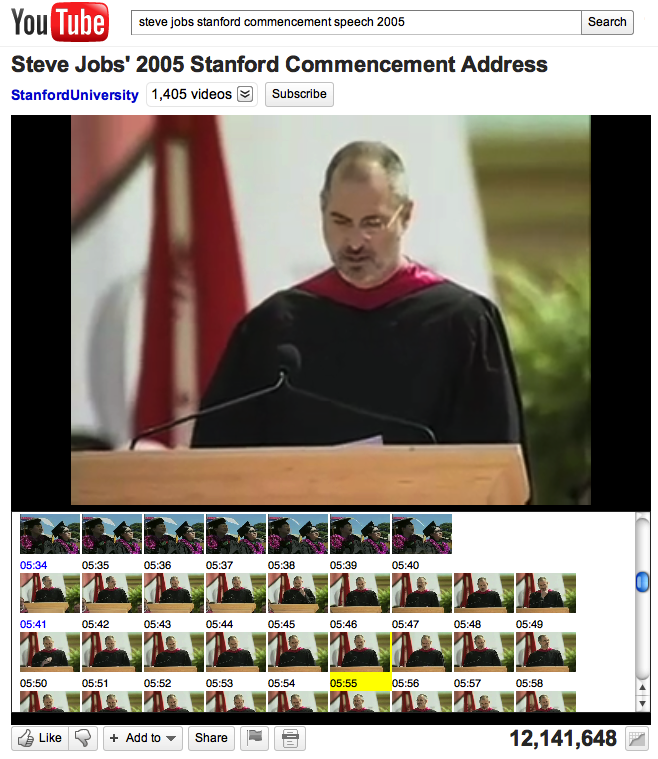
\includegraphics[width=0.7\linewidth]{./stevejobs.png}
  \end{center}
  \caption[Camera shots for a~sample video on  
    a~major online video portal]
    {Camera shots for a~sample video on 
    a~major online video portal, detected on-the-fly via
    our shot boundary algorithm incorporated
    in a~browser extension.}
  \label{fig:screenshot}
\end{figure}

\subsection{Related Work} 
Video fragments consist of shots, which are sequences of
consecutive frames from a~single viewpoint,
representing a~continuous action in time and space.
The topic of shot boundary detection has already been described
extensively in literature.
While some specific issues still remain
(notably detecting gradual transitions and detected false positives
due to large movement or illumination changes),
the problem is considered resolved for many
cases~\cite{yuan2007shotboundary,hanjalic2002shotboundary}.
Below, we present an overview of several well-known categories of shot boundary detection techniques.

\emph{Pixel comparison
methods}~\cite{hampapur1994videosegmentation,
zhang1993videopartitioning} construct a~discontinuity metric
based on differences in color or intensity values
of corresponding pixels in successive frames.
This dependency on spatial location makes this technique
very sensitive to (even global) motion.
Various improvements have been suggested, such as prefiltering
frames~\cite{zhang1995videoparsing},
but pixel-by-pixel comparison methods proved inferior,
which has steered research towards other directions.

A~related method is
\emph{histogram analysis}~\cite{otoole1999shotboundary},
where changes in frame histograms are used
to justify shot boundaries.
Their insensitivity to spatial information
within a~frame makes histograms less prone to partial
and global movements in a~shot.

As a~compromise, a~third group of methods consists of
a~\emph{trade-off between the above two
categories}~\cite{ahmed1999keyframe}.
Different histograms of several, non-overlapping blocks
are calculated for each frame,
thereby categorizing different regions of the frame
with their own color-based, space-invariant fingerprint.
The results are promising, while computational complexity
is kept to a~minimum, which is why we have chosen
a~variation of this approach for our own algorithm.

Other approaches to shot boundary detection include
the \emph{comparison of mean and standard deviations}
of frame intensities~\cite{lienhart1999comparison}.
Detection using other features such as
edges~\cite{zabih1995scenebreaks} and
motion~\cite{bouthemy1997shotchange} have also been proposed.
However, Gargi \emph{et~al.} have shown that
these more complex methods do not necessarily
outperform histogram-based approaches~\cite{gargi2000videoshot}.
A~detailed comparison can be found in
Yuan~\emph{et~al.}~\cite{yuan2007shotboundary}.

\subsection{Shot Boundary Detection Algorithm}
\label{sec:details-of-algo}

In this section, we discuss our shot boundary detection algorithm,
which falls in the category of histogram-based algorithms.
Since visually dissimilar video frames
can have similar global histograms,
we take local histograms into account instead. 
We therefore split video frames in freely configurable
rows and columns, \emph{i.e.}, lay a~grid of tiles over each frame.
The user interface, as can be seen in \autoref{fig:algorithm},
currently allows for anything from a~$\mathit{1} \times \mathit{1}$ 
grid to a~$\mathit{20} \times \mathit{20}$ grid.
The limits are imposed by still reasonable processing time on consumer PCs.
For each step, we examine a~frame $\mathit{f}$ and its direct
predecessor $\mathit{f - 1}$.

Apart from the per-tile average histogram distance,
the frame distance function further considers
a~freely configurable number of \emph{most different} and
\emph{most similar} tiles.
This is driven by the observation that different parts
of a~video have different intensities of color changes,
dependent on the movements from frame to frame.
The idea is thus to boost the influence of movements in the frame
distance function, and to limit the influence of permanence.
In the debug view of our approach, as depicted in
\autoref{fig:algorithm}, blue boxes indicate movements,
while red boxes indicate permanence.
In the concrete example, Steve Jobs' head and shoulders move
as he talks, which can be clearly seen
at the blue boxes in the particular tiles.
Additional movements come from a~swaying flag on the left,
and a~plant on the right.
In contrast, the speaker desk, the white background,
and the upper part of his body remain static,
resulting in red boxes.
We use a~grid layout of $\mathit{20} \times \mathit{20}$ tiles
($\mathit{nTiles} = \mathit{400}$), and
a~$\mathit{tileLimit = 133 = \mathit{20} \times \mathit{20} * 1/3}$
of most different or similar tiles,
\emph{i.e.}, we treat one third of all tiles
as most different tiles, one third as normal tiles,
and one third as most similar tiles,
and apply boosting and limiting factors to the most different
and most similar tiles respectively.
We work with values of~$\mathit{1.1}$ for the
$\mathit{boostingFactor}$, which slightly increases
the impact of the most different tiles,
and $\mathit{0.9}$ for the $\mathit{limitingFactor}$,
which slightly decreases the impact of the most similar tiles.
These algorithm parameters were empirically determined
to deliver solid results on a~large corpus of videos,
albeit for each individual video the optimal settings
can be manually tweaked to take into account the
particular video's special characteristics.
The algorithm pseudo code can be seen in \autoref{code:algorithm}.

We define the average histogram distance between two frames
$\mathit{f}$ and $\mathit{f - 1}$ as $\mathit{avgHisto_{f}}$.
In a~first step, we have examined the histogram distance
data statistically, and observed that while
the overall average frame distance $\mathit{avgDist_{f}}$,
defined as $$\mathit{avgDist_{f}} =
\frac{1}{\mathit{nTiles}}\sum_{t=1}^{\mathit{nTiles}}
\mathit{avgHisto_{f, t}}$$ is very intuitive to human beings,
far more value lies in the standard deviation
$\mathit{stdDev_{f}}$, based on the definition of the overall
average frame distance $\mathit{avgDist_{f}}$
$$\mathit{stdDev_{f}} =
\sqrt{\frac{1}{\mathit{nTiles}}\sum_{t=1}^{\mathit{nTiles}}
(\mathit{avgHisto_{f, t}} - \mathit{avgDist_{f}})^{2}}$$
We use the standard deviation as a~value for the shot splitting
threshold~\cite{lienhart1999comparison}
to obtain very accurate shot splitting results.
We found the boosting and limiting factors to have an overall
positive quality impact on more lively videos,
and a~negative quality impact on more monotone videos.
Best results can be achieved if,
after changing either the boosting or the limiting factors
for the most similar or different tiles,
the value of the shot splitting threshold is adapted
to the new resulting standard deviation.
The user interface can do this automatically.

\begin{figure}
  \begin{center}
    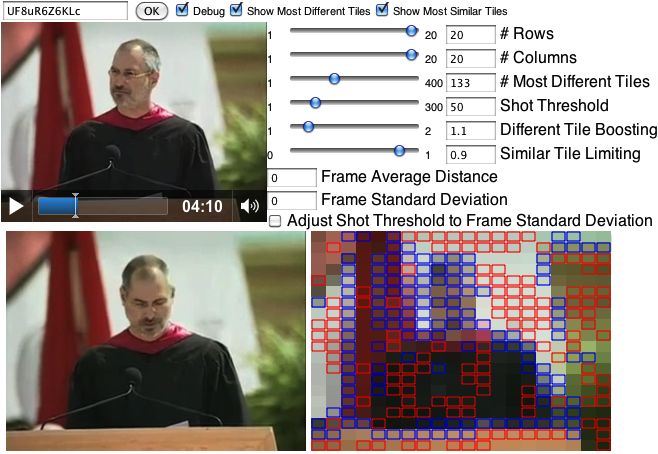
\includegraphics[width=1.0\linewidth]{./algorithm.png}
  \end{center}
  \caption[Debug view of the shot boundary detection process]
    {Debug view of the shot boundary detection process.
    Blue boxes highlight tiles with most differences
    to the previous frame, red boxes those with most similarities.}
  \label{fig:algorithm}
\end{figure}

\begin{lstlisting}[caption=Pseudocode of the shot boundary detection
  algorithm,
  label=code:algorithm, float]
for frame in frames
  f = frame.index  
  for tile in tiles of frame      
    avgHisto[f][tile] = getTilewiseDiff()
 
  mostDiffTiles = getMostDiffTiles(avgHisto[f])
  mostSimTiles = getMostSimTiles(avgHisto[f])
 
  for tile in tiles of frame    
    factor = 1  
    if tile in mostDiffTiles
      factor = boostingFactor
    else if tile in mostSimTiles
      factor = limitingFactor
    avgHisto[f][tile] = avgHisto[f][tile] * factor
  avgDist[f] = avg(avgHisto[f])
\end{lstlisting}

\subsection{Implementation Details}
\label{sec:implementation}

The complete video analysis process happens fully
on the client side.
We use the HTML5 JavaScript APIs of the \texttt{<video>} and
\texttt{<canvas>} tags.
In order to obtain a~video still frame
from the \texttt{<video>} tag at the current video position,
we use the \texttt{drawImage()} function of the 2D context of the
\texttt{<canvas>} tag,
which accepts a~video as its first parameter.
We then analyze the video frame's pixels tile-wise
and calculate the histograms.
In order to retrieve the tile-wise pixel data
from the 2D context of the \texttt{<canvas>},
we use the \texttt{getImageData()} function.
For processing speed reasons, we currently limit our approach to
a~resolution of one second, \emph{i.e.},
for each analysis step,
seek the video in $\mathit{1s}$ steps.
We then calculate the frame distances as outlined in
\autoref{sec:details-of-algo}.
For each frame, we can optionally generate an \texttt{<img>} tag
with a~base64-encoded data URI representation
of the video frame's data
that can serve for filmstrip representations of the video.

\subsection{Evaluation}

Detecting shots on-the-fly in streaming video
comes with its very own challenges.
First, it is a~question of streaming speed.
Especially with high-definition (HD) video,
this can be very demanding.
We do not attach the analysis \texttt{<video>} tag
to the DOM tree~\cite{lehors2004dom} to save some CPU cycles,
however, the video playing logic still has to seek the video position
ahead in one-second steps  and process the encountered still frame.
Even on a~higher-end computer (our experiments ran on a~MacBook
Pro, Intel Core 2 Duo 2,66 GHz, 8 GB RAM),
the process of analyzing and displaying in parallel
a~$\mathit{1280} \times \mathit{720}$ HD video of media type
\emph{video/mp4; codecs="avc1.64001F, mp4a.40.2"}
caused an average CPU load of about 70\%.
The HTML5~\cite{berjon2012html5} specification states that
\textit{``when the playback rate is not exactly 1.0,
hardware, software, or format limitations can cause video frames
to be dropped''}.
In practice, this causes the analysis environment
to be far from optimal.
In our experiments we differentiated between false positives,
\emph{i.e.}, shot changes that were detected,
but not existent, and misses, \emph{i.e.},
shot changes that were existent,
but not detected.
Compared to a~set of videos with manually annotated shot changes,
our algorithm detected fewer false positives than misses.
The reasons were gradual transitions and shots
shorter than one second (below our detection resolution)
for misses, and large movements in several tiles
for false positives.
Overall, we reached an accuracy of about 86\%,
which is not optimal, but given the challenges
sufficient for our use case of
detecting near- or exact duplicate videos. 

\subsection{Optimization Potential}

Optimization potential lies in
improving the analysis speed by dynamically selecting
lower quality analysis video files,
given that videos are oftentimes available in several resolutions,
like Standard Definition (SD) or High Definition (HD).
We have checked in how far analysis results differ
for the various qualities,
with the result that SD quality is sufficient.
We have made available the shot detection application online at
\url{http://tomayac.com/youpr0n/} and invite the reader to compare
the results, \emph{e.g.}, the SD video
\url{http://tomayac.com/youpr0n/videos/vsfashionshow_sd.mp4} with
the HD version \url{http://tomayac.com/youpr0n/videos/vsfashionshow_hd.mp4}.

Second, more advanced heuristics for the various user-definable
options in the analysis process are needed.
While there is no optimal configuration for all types of videos,
there are some key indicators that can help categorize videos
into classes and propose predefined known working settings
based on the standard deviation $\mathit{stdDev_{f}}$
and the overall average frame distance $\mathit{avgDist_{f}}$.
Both are dependent on the values of $\mathit{boostingFactor}$,
$\mathit{limitingFactor}$, $\mathit{rows}$, and $\mathit{columns}$. 
Interpreting our results, there is evidence
that low complexity settings are sufficient in most cases,
\emph{i.e.}, a~number of $\mathit{rows}$ and $\mathit{columns}$
higher than~$\mathit{2}$ does not necessarily
lead to more accurate shot boundary detection results.
The same applies to the number of to-be-considered most different
or similar tiles $\mathit{tileLimit}$.
We had cases where not treating those tiles differently
at all, \emph{i.e.}, setting
$\mathit{boostingFactor} = \mathit{limitingFactor} = \mathit{1}$, 
led to better results; for example with screencast-type videos,
typically used to demonstrate and teach the use of software features,
that were not recorded with a real camera,
but directly recorded from the computer's screen, with ``camera shots''
then later added with video editing software.

\section{Photo Deduplication}

We determine the popularity of media items
shared across social networks.
This task involves the deduplication of extracted media items.
In the previous section, we have presented an algorithm
for on-the-fly shot boundary detection for video media items.
In this section, we will show how components of this algorithm
can be used to deduplicate photos.

\subsection{Problem Statement}
\label{sec:problem-statement}

Our work is situated in the broader context of summarizing events
based on social network data.
In order to get an overview of a~given event based on a~\emph{potentially huge} set
of event-related media items, this set of media items needs to be \emph{pruned}
to exclusively contain highly relevant media items that are as representative
for the event as possible.
Rather than showing the viewer all media items,
clusters of similar media items need to be formed.
Within each cluster, the most representative media item
has to be recognized as such, according to well-defined criteria.
Undesired duplicate or near-duplicate content in the context of social networks
arises in a~number of situations
that we will illustrate in the following.
All shown examples of media items were actually shared on social networks
and were clustered correctly as near-duplicates
by our clustering algorithm, which we will detail in
\autoref{sec:near-duplicate-clustering-algorithm}.
First, we look at related work for the task of photo deduplication.

\subsection{Related Work}

\paragraph{Image Deduplication and Clustering}

Work on ordinal measures that serve as a~general tool for
image matching was performed by Bhat \emph{et al.}\
in~\cite{bhat1998imagecorrespondence}.
Chum \emph{et al.}\ have proposed a~near-duplicate image detection method
using min-Hash and term frequency--inverse document frequency (tf--idf)
weighting~\cite{chum2008nearduplicate}.
They use a~visual vocabulary of vector quantized local feature descriptors based on
Scale-Invariant Feature Transform (SIFT)~\cite{lowe1999sift}.
Gao \emph{et al.}~\cite{gao2005webimageclustering} have proposed an image clustering method
in the context of Web image clustering, which clusters images
based on the consistent fusion of the information contained in
both low-level features and surrounding texts.
Also in the context of Web pages, Cai
\emph{et al.}~\cite{cai2004hierarchicalclustering} have proposed
a~hierarchical clustering method using visual, textual, and link analysis.
Goldberger \emph{et al.}~\cite{goldberger2006unsupervisedclustering} 
have combined discrete and continuous image models based on a~mixture of Gaussian densities
with a~generalized version of the information bottleneck principle
for unsupervised hierarchical image set clustering. 
Chen \emph{et al.}~\cite{chen2003cbir} have introduced an image retrieval approach,
which tackles the semantic gap problem by learning similarities
of images of the same semantics.

\subsection{Duplicate Content}
\label{sec:duplicate-content}

Duplicate content in the context of social networks
arises whenever people either share exactly the same,
or an exact copy of a~given media item.
An example of the latter can be one user uploading the same media item
to the two different social networks \googleplus and Facebook,
and an example of the prior can be two users sharing the same
YouTube video independently from each other, or re-sharing each other's content.

\subsubsection{Near-Duplicate Content}

Near-duplicate content in the context of social networks
arises in a~number of situations
that we will illustrate in the following.
All photos are real examples of media items shared on social networks
that were clustered correctly as near-duplicates
by our clustering algorithm, which we will detail in
\autoref{sec:near-duplicate-clustering-algorithm}.

\paragraph{Different Viewing Angle}

When two people attend the same event
and create media items at roughly the same time
and covering the same scene,
their media items will be similar
and---the capturing devices' qualities aside---only differ in the viewing angle. 
\autoref{fig:viewing-angle} shows a~concrete example.

\begin{figure}[h!]
  \centering
  \subfloat[Viewing angle 1]{
    
\includegraphics[width=0.3\textwidth]{stage1.jpg}
  }                
  \subfloat[Viewing angle 2]{
    
\includegraphics[width=0.3\textwidth]{stage2.jpg}
  }
  \caption{Slightly different viewing angles of a~concert stage.}
  \label{fig:viewing-angle}  
\end{figure}

\paragraph{Logo, Watermark, Lower Third, or Caption Insertion}

Oftentimes, organizations or individuals insert
logos, watermarks, lower thirds, or captions into media items
to highlight their origin, to convey related information,
or to claim ownership of a~media item.
An example of caption, logo, and lower third insertion
can be seen in \autoref{fig:logo}.

\begin{figure}[h!]
  \centering
  \subfloat[Blank]{
    
\includegraphics[width=0.25\textwidth]{speaker1.jpg}
  }                
  \subfloat[Caption]{
    
\includegraphics[width=0.25\textwidth]{speaker2.jpg}
  }
  \subfloat[Logo, lower third]{
    
\includegraphics[width=0.25\textwidth]{speaker3.jpg}
  }
  \caption{Caption, logo, and lower third insertion for a~speaker.}
  \label{fig:logo}  
\end{figure}

\paragraph{Cropping}

Cropping refers to the removal of the outer parts of a~media item
to improve framing, accentuate subject matter,
or to (lossily) change the aspect ratio.
Cropping either happens manually via an image editing application,
or, more often, by the social networks themselves
to obtain a~square aspect ratio
that better fits the timeline view of users,
as can be seen in the example in \autoref{fig:cropping}.

\begin{figure}[h!]
  \centering
  \subfloat[Original]{
    
\includegraphics[width=0.26\textwidth]{kid1.jpg}
  }                
  \subfloat[Cropped]{
    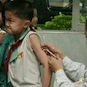
\includegraphics[width=0.18\textwidth]{kid2.jpg}
  }
  \caption[Original and cropped version of a~photo]
  {Original and cropped version of a~photo (including a~slight color variation).}
  \label{fig:cropping}  
\end{figure}

\paragraph{Different Keyframes}

We have shown an approach to camera shot boundary detection in~\cite{steiner_www_2012b}.
Different frames stemming from the same camera shot
can occur on social networks, when preview heuristics
attempt to auto-select a~well-identifying poster frame from a~video with different approaches,
typically resulting in different frames for different social networks.
\autoref{fig:camera-shot} shows an example of this phenomenon.

\begin{figure}[h!]
  \centering
  \subfloat[Frame 1]{
    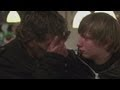
\includegraphics[width=0.2\textwidth]{camera1.jpg}
  }                
  \subfloat[Frame 2]{
    
\includegraphics[width=0.2\textwidth]{camera2.jpg}
  }
  \caption[Two different frames stemming from the same camera shot]
    {Two different frames stemming from the same camera shot,
    with the left photo appearing slightly earlier in the video.}
  \label{fig:camera-shot}  
\end{figure}

\paragraph{Aspect Ratio Changes with Squeezing or Stretching}

Aspect ratio changes can either happen combined with cropping
(and thus losing parts of the media item), and/or combined with 
squeezing or stretching (and thus deforming the media item).
\autoref{fig:stretched} shows an example where a~media item gets stretched.

\begin{figure}[h!]
  \centering
  \subfloat[Original]{
    
\includegraphics[width=0.155\textwidth]{lordoftherings.jpg}
  }                
  \subfloat[Stretched]{
    
\includegraphics[width=0.3\textwidth]{lordoftheringsstretched.jpg}
  }
  \caption{Original, and stretched version of a~photo.}
  \label{fig:bulged}  
\end{figure}

\paragraph{Photo Filters}

With the raising popularity of Instagram with its 90 million monthly active users%
\footnote{\url{http://instagram.com/press/}, accessed 02/14/2013},
photo filters that, \emph{e.g.}, emulate retro Polaroid\texttrademark\ or tilt-shift effects,
are a~considerable reason for near-duplicate media content on social networks.
\autoref{fig:photo-filter} shows a~typical example.

\begin{figure}[h!]
  \centering
  \subfloat[Original]{
    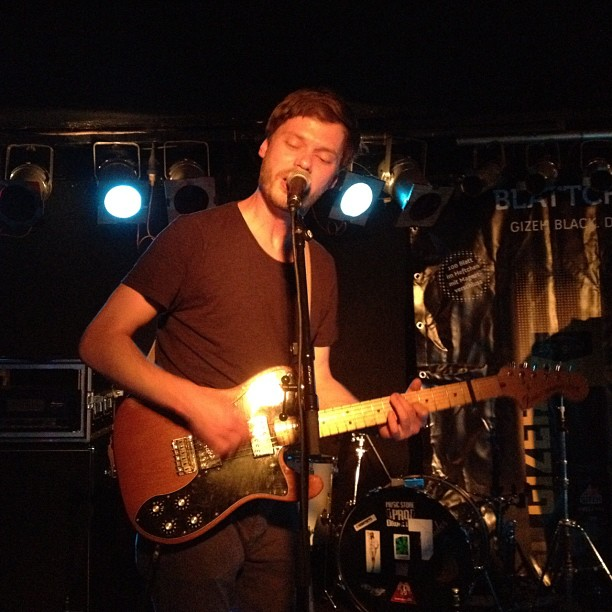
\includegraphics[width=0.25\textwidth]{clickclickdecker1.jpg}
  }                
  \subfloat[With photo filter]{
    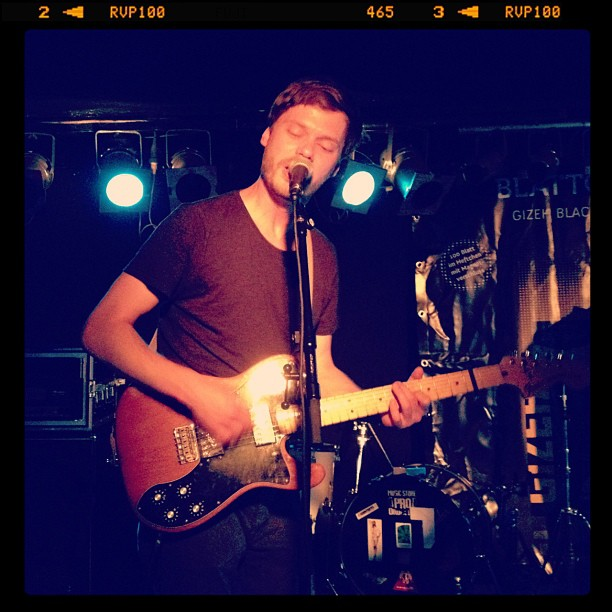
\includegraphics[width=0.25\textwidth]{clickclickdecker2.jpg}
  }
  \caption{Original, and version with an applied photo filter of a~photo.}
  \label{fig:photo-filter}  
\end{figure}

\subsection{Near-Duplicate Photo Clustering Algorithm}
\label{sec:near-duplicate-clustering-algorithm}

In this subsection, we detail our near-duplicate photo clustering algorithm
and its design goals.
We start with a~description of its face detection component.

\subsection{Face Detection}
\label{sec:face-detection}

Face detection is a~computer vision technology
that determines the regions of faces in media items.
Rotation-invariant face detection aims to detect faces with arbitrary
rotation angles and is crucial as the first step in automatic face detection
for general applications, as face images on social media are seldom upright and frontal.
Face detection is a~subclass of the broader class of object detection.
The Viola--Jones object detection framework proposed in 2001
by Paul Viola and Michael
Jones~\cite{viola2001objectdetection,viola2004robust}
provides competitive object detection rates in realtime
and was motivated primarily by the problem of face detection.
We use an algorithm that further improves Viola--Jones,
based on work by Huang \emph{et al.}~\cite{huang2007facedetection}
and Abramson \emph{et al.}~\cite{abramson2007yef},
in a~JavaScript implementation made available by Liu~\cite{liu2012facedetection}.
This algorithm is fast enough to be applied to hundreds of media items
in well less than a~second overall processing time on a~standard laptop
(mid-2010 MacBook~Pro).

\subsection{Algorithm Description}

Our near-duplicate media item clustering algorithm belongs to the family of
tile-wise histogram-based clustering algorithms.
As an additional semantic feature, the algorithm considers detected faces
as described above.
For two media items to be clustered,
the following conditions have to be fulfilled.

\begin{enumerate}
  \item Out of $m$ tiles of a~media item with $n$ tiles ($m \leq n$),
    at most $\textit{tiles\_threshold}$ tiles may differ not more than $\textit{similarity\_threshold}$
    from their counterpart~tiles.
  \item The numbers $f_1$ and $f_2$ of detected faces in both media items
    have to be the same.
    We note that we do not \emph{recognize} faces, but only \emph{detect} them.
\end{enumerate}

The simplified algorithm pseudocode can be seen in \autoref{code:clustering}.
In the actual implementation, some speed improvements,
like, for example, looking up already calculated
distances\footnote{\texttt{distances[outerItem][innerItem] =
distances[innerItem][outerItem]}}
have been applied;
these were omitted in the listing for legibility reasons.
We calculate the histograms and distances only once initially.
The clusters are then recalculated dynamically
whenever either $\textit{tiles\_threshold}$ or $\textit{similarity\_threshold}$ change.
The given values of $\textit{rows} = \textit{cols} = 10$ and
$\textit{tiles\_threshold} = 67 = \lceil \textit{rows} \cdot \textit{cols} \cdot 2/3 \rceil$
and $\textit{similarity\_threshold} = 10$ were determined empirically
on a~large corpus of event-related media items
and are known to deliver solid results.
The corpus has been made available publicly,
see \autoref{sec:evaluation-chpater6} for the details.

\begin{lstlisting}[float=top,caption={Simplified pseudocode of the exact- and near-duplicate media item deduplication and clustering algorithm},
  label={code:clustering},escapechar=§]
§\textbf{Input:}§ mediaItems, a~list of media items
§\textbf{Output:}§ clusters, a~list of clustered media items

§\textbf{init:}§


§\textit{\# Algorithm settings}§
ROWS = 10
COLS = 10
TILES_THRESHOLD = ceil(ROWS * COLS * 2/3)
SIMILARITY_THRESHOLD = 10


§\textit{\# Calculates tile-wise histograms}§
histograms = {}
faces = {}
§\textbf{for}§ item §\textbf{in}§ mediaItems
  faces[item] = getFaces(item)
  
  histograms[item] = {}
  §\textbf{for}§ tile §\textbf{in}§ item
    histograms[item][tile] = getHistogram(tile)
  §\textbf{end for}§
§\textbf{end for}§  

    
§\textit{\# Calculates tile-wise distances}§
distances = {}
§\textbf{for}§ outerItem §\textbf{in}§ mediaItems
  distances[outerItem] = {}
  §\textbf{for}§ innerItem §\textbf{in}§ mediaItems
    distances[outerItem][innerItem] = {}
    §\textbf{for}§ tile §\textbf{in}§ histograms[outerItem]
      distances[outerItem][innerItem][tile] =
          abs(histograms[outerItem][tile] -
              histograms[innerItem][tile])
    §\textbf{end for}§
  §\textbf{end for}§
§\textbf{end for}§

  
§\textit{\# Calculates clusters}§
clusters = {}
§\textbf{for}§ outerItem §\textbf{in}§ mediaItems  
  clusters[outerItem] = []  
  §\textbf{for}§ innerItem §\textbf{in}§ mediaItems
    §\textbf{if}§ outerItem == innerItem §\textbf{then}§ continue
    
    similarTiles = 0
    distance = distances[outerItem][innerItem]
    §\textbf{for}§ tile §\textbf{in}§ distance      
      §\textbf{if}§ distance[tile] <= SIMILARITY_THRESHOLD §\textbf{then}§
        similarTiles++
      §\textbf{end if}§
    §\textbf{end for}§
         
    §\textit{\# Check condition 1 (tiles)}§
    §\textbf{if}§ similarTiles >= TILES_THRESHOLD §\textbf{then}§
      §\textit{\# Check condition 2 (faces)}§
      §\textbf{if}§ faces[outerItem] == faces[innerItem] §\textbf{then}§
        clusters[outerItem].push(innerItem)
      §\textbf{end if}§
    §\textbf{end if}§    
  §\textbf{end for}§
§\textbf{end for}§

§\textbf{return}§ clusters        
\end{lstlisting}

\subsection{Experiments}

We have evaluated the near-duplicate photo clustering
on two events from recent history with high social network coverage
that we will briefly describe in the following.

\subsubsection{Grammy Awards Nominations 2013}

The Grammy Award---or short Grammy---is an award by
the National Academy of Recording Arts and Sciences of the United States
to recognize outstanding achievement in the music industry.
The annual ceremony features performances by prominent artists,
and some of the awards are presented in a~widely viewed televised ceremony.
On December 5, 2012, the nominees for the 55\superscript{th} Annual Grammy Awards
were announced at an event broadcasted live by CBS
titled \emph{Grammy Nominations Concert
Live}\footnote{\url{http://en.wikipedia.org/wiki/2013_Grammy_Awards},
accessed December 7, 2012},
during which Taylor Swift and LL~Cool~J revealed the nominees in several key categories, including the so-called Big Four: Album, Record and Song of the Year and Best New Artist.
CBS suggested the hashtag \texttt{\#GRAMMYNoms} for the event.

\subsubsection{Victoria's Secret Fashion Show 2012}

The \emph{Victoria's Secret Fashion
Show}\footnote{\url{http://en.wikipedia.org/wiki/Victoria's_Secret_Fashion_Show},
accessed December 7, 2012} is an annual event
sponsored by Victoria's Secret, a~brand of lingerie and sleepwear.
The show features some of the world's leading fashion models
and is used by the brand to promote and market its goods in high-profile settings.
American network television broadcasts the show during prime time.
The show is a~lavish event with elaborate costumed lingerie and
varying music by leading entertainers
that attracts hundreds of celebrities and entertainers,
with special performers and acts every year.
The 2012 edition of the show,
which was previously taped on November 7, 2012
was aired on December 4, 2012 on CBS
to an audience of 9.48 million viewers.
CBS suggested the hashtag \texttt{\#VSFashionShow} for the event.

\subsection{Algorithm Debug View}
\label{sec:algorithm-debug-view}

In order to illustrate the way the algorithm clusters media items,
\autoref{fig:algorithmdebug} shows a~debug view of the algorithm
for two clustered media items related to the 
\emph{Grammy Awards Nominations 2013} event.
The red border around the media item indicates at least one detected face.
Independent from the actual media item's aspect ratio,
the tile-wise comparison always happens based on a~potentially squeezed
square aspect ratio version.
The two slightly different media items (caption insertion, lighting change)
were clustered, because out of the $10 \cdot 10 = 100$ tiles,
$85$ of the minimum required $\textit{tiles\_threshold}$ of $67$ tiles differed not more
than the $\textit{similarity\_threshold}$ of $10$ per tile.
In both media items, exactly $1$ face was detected.
A~screenshot of the complete media item clustering application (with a~different event)
is available online at \url{http://twitpic.com/c02qfs/full} (accessed 02/14/2013).

\begin{figure}
  \centering
  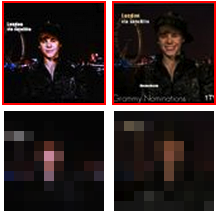
\includegraphics[width=0.5\linewidth]{./algorithmdebug.png}
  \caption[Algorithm debug view for two clustered media items]
  {Algorithm debug view for two clustered media items related to the \emph{Grammy Awards Nominations 2013} event (the red border around the media items indicates at least one detected face)}
  \label{fig:algorithmdebug}
\end{figure}
\subsection{Evaluation}\label{sec:evaluation-chpater6}

We have collected and made available%
\footnote{\url{https://www.dropbox.com/sh/2llvjaut32juwrx/7eGLodfP_2},
accessed February 12, 2013}
datasets for both events with
379 photos for the \emph{Victoria's Secret Fashion Show 2012} event 
and 949 photos for the \emph{Grammy Awards Nominations 2013} event.
These photos were collected using the media item extraction framework
described in \autoref{cha:media-item-extraction}
using a~mix of hashtag searches with the official event hashtags combined
with full-text searches for event titles and variations thereof.
Due to the short-lived nature of social networks,
the returned results of the media item extraction process itself
are not reproducible; our focus in this chapter
is on media item deduplication and clustering.
The concrete clustering parameters for the algorithm were set as listed below.

\begin{enumerate}
  \item $\textit{rows}$ = $\textit{cols}$ = $10$
  \item $\textit{tiles\_threshold}$ = $67$
  \item $\textit{similarity\_threshold}$ = $10$
\end{enumerate}

In the following, we discuss the clustering and deduplication results.
\autoref{fig:topvsfashionshow} and \autoref{fig:topgrammy} show the top clusters
for the \emph{Victoria's Secret Fashion Show 2012} and the 
\emph{Grammy Awards Nominations 2013} events respectively.
We will then pick some representative examples from both events
and have a~closer look at the clustering algorithm's strengths and weaknesses.

\begin{figure}[h!]
  \centering
  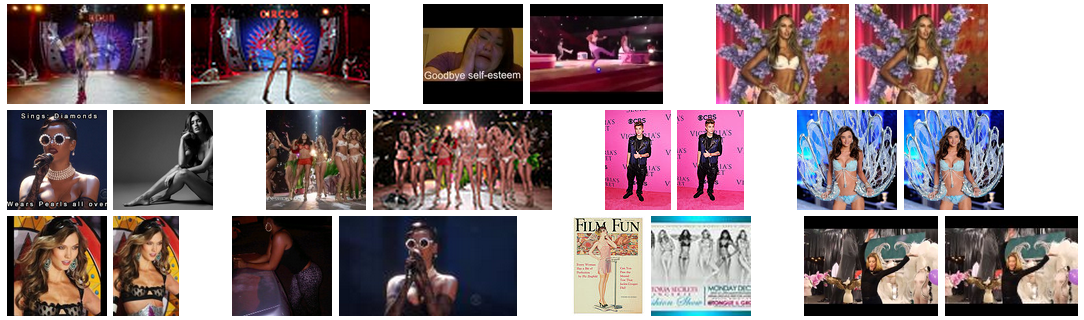
\includegraphics[width=1.0\linewidth]{./vsfashionshow_clusters.png}
  \caption{Top clusters for the \emph{Victoria's Secret Fashion Show 2012} event}
  \label{fig:topvsfashionshow}
\end{figure}

\begin{figure}[h!]
  \centering
  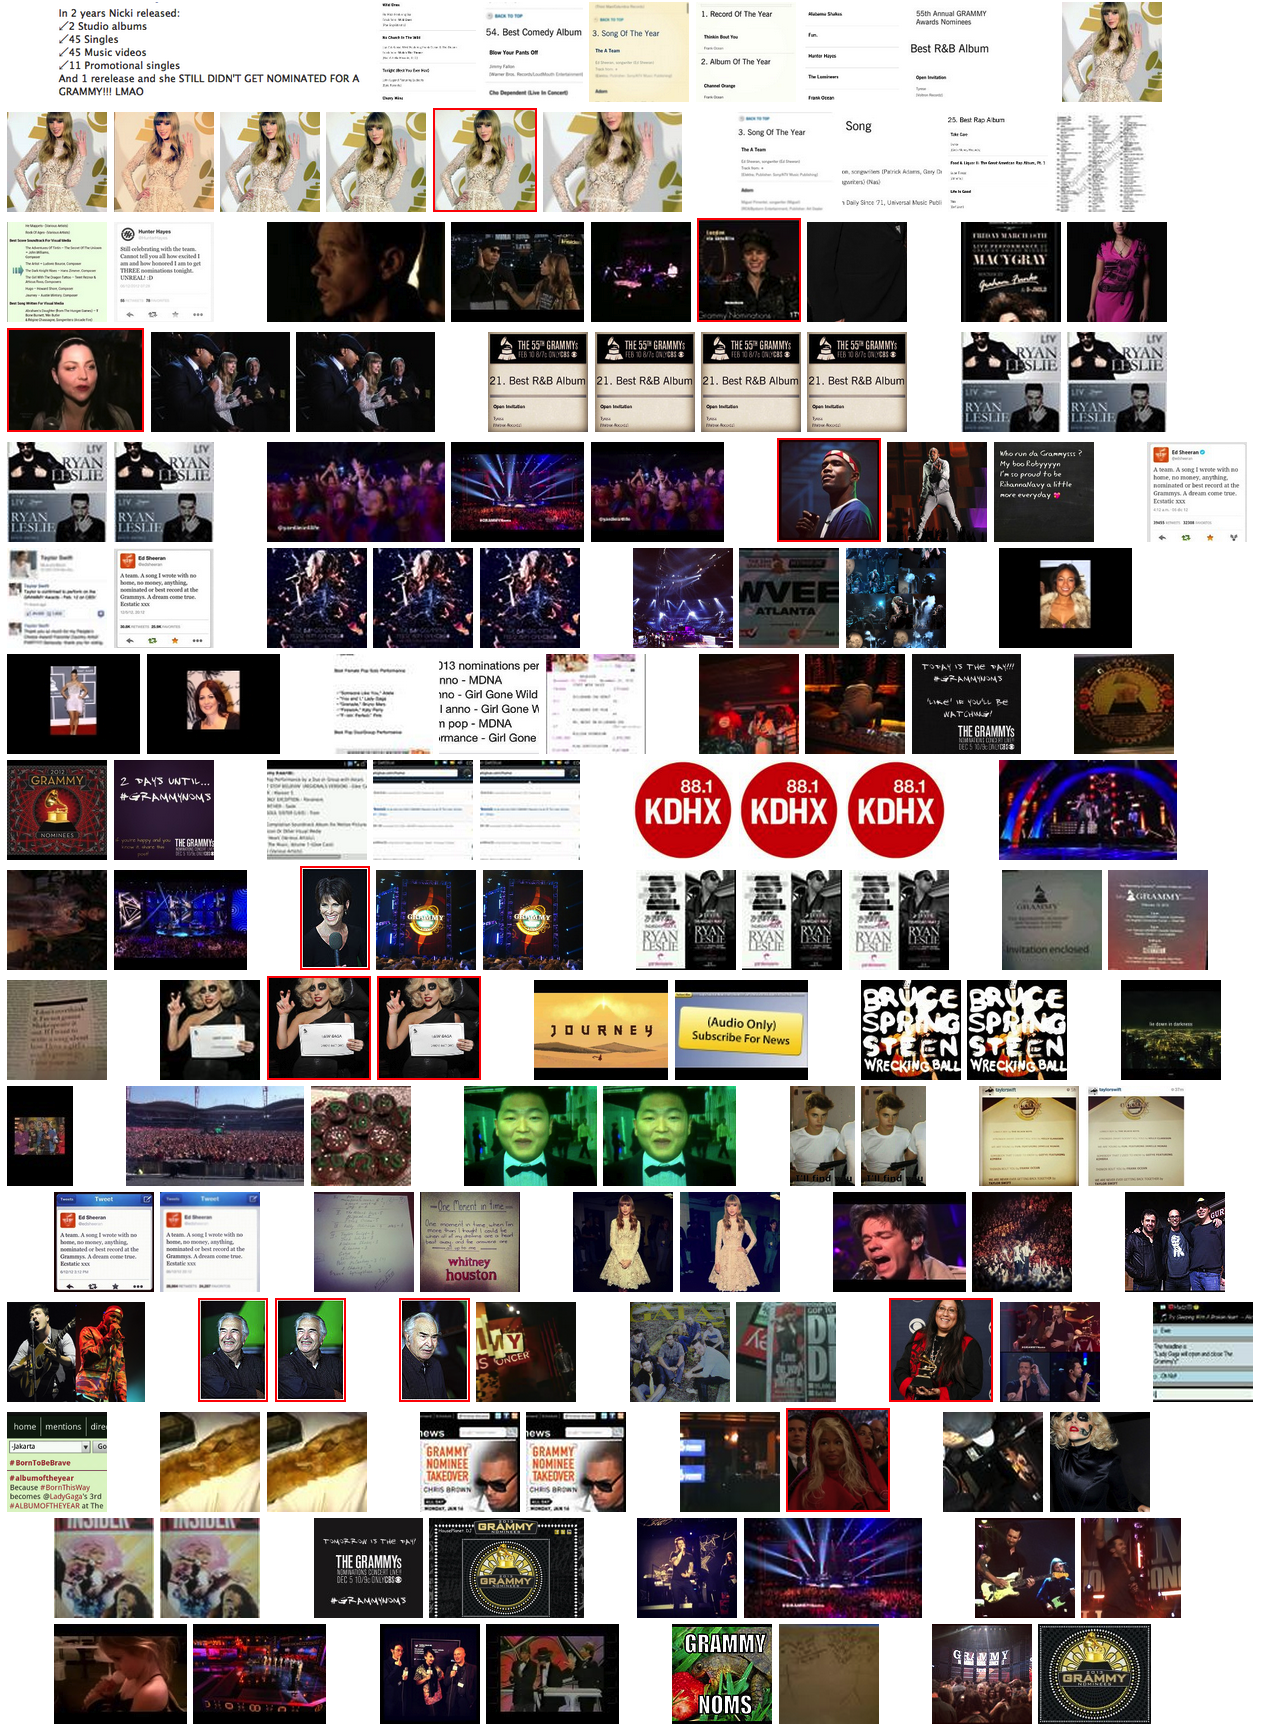
\includegraphics[width=0.97\linewidth]{./grammy_clusters.png}
  \caption{Top clusters for the \emph{Grammy Awards Nominations 2013} event}
  \label{fig:topgrammy}
\end{figure}

\subsubsection{Algorithm Strengths} 

\autoref{fig:personclose} has a~brunette fashion model in a~pink robe
and a~heart-shaped pink spotlight as central elements of both photos. 
Even though the model is shot from different angles and at different times,
the photos are successfully clustered due to the very identifying colors
and the high tile similarity. 

\begin{figure}[h!]
  \centering
  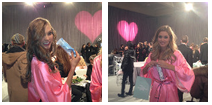
\includegraphics[width=0.4\linewidth]{./person.png}
  \caption{High tile-wise similarity of a~dominating color}
  \label{fig:personclose}
\end{figure}

\autoref{fig:scenecrop} shows two different views of a~stage
taken at slightly different times.
The left photo covers a~detail of the scene,
whereas the right photo covers the entire stage.
Due to the high tile-wise similarity of the scene detail,
the photos are successfully clustered.

\begin{figure}[h!]
  \centering
  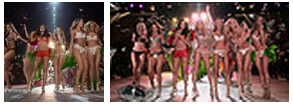
\includegraphics[width=0.5\linewidth]{./scene.png}
  \caption{Cropped view of a~stage scene}
  \label{fig:scenecrop}
\end{figure}

\autoref{fig:lightingconditions} shows two views of a~stage
under different lighting conditions.
Due to the tile color tolerances and the high tile-wise similarity,
the photos are successfully clustered.

\begin{figure}[h!]
  \centering
  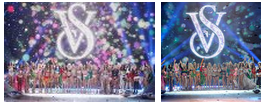
\includegraphics[width=0.5\linewidth]{./viewing_angle.png}
  \caption{Stage and detail of a~stage under different lighting conditions}
  \label{fig:lightingconditions}
\end{figure}

\autoref{fig:zoomed} shows two photos of the same model
where the left photo is a~zoomed version of the right photo 
with added black bars so that the resulting photo
has a~square aspect ratio.
Despite the differences, the photos are successfully clustered.

\begin{figure}[h!]
  \centering
  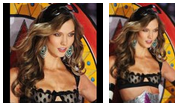
\includegraphics[width=0.35\linewidth]{./zoom.png}
  \caption{Zoomed view of a~model with black bars left and right}
  \label{fig:zoomed}
\end{figure}

\autoref{fig:stageperson} shows two views of the same stage,
however, with a~different person.
Due to the dominating tile-wise similarity of the stage tiles,
the photos are correctly clustered.

\begin{figure}[h!]
  \centering
  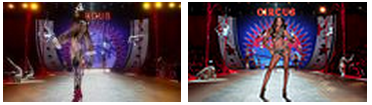
\includegraphics[width=0.6\linewidth]{./stage.png}
  \caption{Two views of the same stage with different person}
  \label{fig:stageperson}
\end{figure}

\subsubsection{Algorithm Weaknesses}

\autoref{fig:white} shows five media items with pure white
as the dominating color and a~pure black font,
where users had taken screenshots of the Grammy results from Web pages.
The algorithm in its previously described form clusters such media items.
This may or may not be desired.
Likewise at the other end of the color spectrum,
\autoref{fig:bwtolerance} shows two media items of a~woman
with pure black as the dominating color,
one time with, and the other time without added black bars
to fit a~letterbox aspect ratio.
In its previously described form, the algorithm
does \emph{not} cluster such media items
(unless a~really small number $\textit{tiles\_threshold}$ 
of required similar tiles is selected).

In the majority of cases, though, clustering such media items \emph{is} desired.
Our response to both issues is to ignore a~certain part
of the color spectrum in the algorithm's similarity measure.
In the concrete case, ignoring pure white and pure black correctly fixed
the clustering in our chosen example events in all but one cases,
without negatively impacting previously correctly formed clusters.

Finally, \autoref{fig:weakness} shows two entirely different media items
that were incorrectly clustered as the tile histograms
were similar enough under the chosen similarity threshold.
The explanation for this is twofold.
First, the original source media items were very small thumbnail-like images,
which hindered face recognition
(there is actually an \emph{unequal} number of faces in each image).
Second, the way the algorithm works,
which is best understood by looking at \autoref{fig:algorithmdebug},
causes the tiles of very tiny media items like the ones in question to blur.

We have experienced in our experiments that there is no single perfect
combination of algorithm parameters,
so the only way to address this issue (besides ignoring too small media items,
which in practice may be the easiest and best solution)
is to make the parameters flexible.
In our graphical user interface we have created sliders
that let the user interactively preview clustering changes.
As noted before, a~screenshot of the application
is available online at the URL \url{http://twitpic.com/c02qfs/full}.

\begin{figure}[h!]
  \centering
  
\includegraphics[width=0.8\linewidth]{./white.png}
  \caption{Pure white as dominating color stemming from screenshots}
  \label{fig:white}
\end{figure}

\begin{figure}[h!]
  \centering
  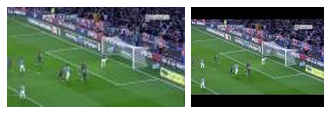
\includegraphics[width=0.55\linewidth]{./bwtolerance.png}
  \caption[Black bars added to fit a~16:9 image in a~4:3 letterbox]
    {Black bars added to fit a~16:9 image in a~4:3 letterbox
    (the white border is part of the original photo)}
  \label{fig:bwtolerance}
\end{figure}

\begin{figure}[h!]
  \centering
  
\includegraphics[width=0.4\linewidth]{./weakness.png}
  \caption{Entirely different photos with similar tile histograms}
  \label{fig:weakness}
\end{figure}

\section{Video Deduplication}

In the previous subsection, we have introduced
an algorithm for photo deduplication.
In the upcoming section, we will outline the conceptual framework
of how this algorithm can be combined with the previously introduced
video shot boundary detection algorithm to on the one hand
directly deduplicate videos on a~shot boundary frame basis,
or to on the other hand detect
whether a~given photo is contained in a~video.

\subsection{Related Work}

\paragraph{Video Deduplication and Clustering}

More specialized methods for video deduplication exist,
for example~\cite{min2011nearduplicatevideo,wu2009nearduplicate}
by Min \emph{et al.}\ who, given the observation that 
transformations tend to preserve the semantic information conveyed
by the video content, propose an approach for identifying
near-duplicate videos by making use of both low-level visual
features and high-level semantic features
detected using trained classifiers.
In~\cite{oliveira2010nearduplicate}, Oliveira
\emph{et al.} report on four large-scale online surveys
wherein they have confirmed that humans perceive videos as near-duplicates
based on both non-semantic features like different photo or audio
quality, but also based on semantic features like different
videos of similar content.
A~survey of video deduplication methods has been conducted by
Lian \emph{et al.}\ in~\cite{lian2010survey}.
In~\cite{guil2007clustering}, Guil \emph{et al.} have proposed a~method
for detecting copies of a~query video in a~videos database
that groups frames with similar visual content while maintaining their temporal order.
In~\cite{okamoto2002videoclustering}, Okamoto \emph{et al.} have proposed an approach
that is based on fixed length video stream segments.
By generating spatio-temporal images, they employ co-occurrence matrices
to express features in the time dimension explicitly. 
Yi \emph{et al.} have proposed motion histograms in~\cite{yi2005motionhistogram},
where the motion content of a~video at pixel level is represented
as a~Pixel Change Ratio Map (PCRM), which captures the motion intensity,
spatial location, and size of moving objects in a~video sequence. 

\paragraph{Image and Video Deduplication and Clustering}

A~method for both photos and videos
has been proposed by Yang \emph{et al.}~\cite{yang2009nearduplicate}.
The authors describe a~system for detecting duplicate images and videos
in a~large collection of multimedia data that uses local difference patterns
as the unified feature to describe both images and videos.
It has been demonstrated that the proposed method is robust against
common image-processing tasks used to produce duplicates.

\subsection{Photo-contained-in-Video Workflow}

In a~first step, for a~given video, we detect shot boundaries
as described before in \autoref{sec:videoshotboundarydetection}.
To illustrate this,
\autoref{fig:vsfashionshowboundaries} shows an excerpt
of detected shot boundaries for a~video related to
the \emph{Victoria's Secret Fashion Show 2012} event.
The first photo of each shot boundary film stripe
is selected as the particular shot's representative photo.
To detect whether a~given photo stemming from social networks
is contained in the video in question,
the set of extracted shot representative photos is compared
with all social network photos,
some of which are shown in \autoref{fig:topvsfashionshow}.
We note, however, that especially for longer videos
(about 4 minutes and longer)
this approach does not scale due to the sheer number of shot boundaries
in common videos shared on social networks,
which causes the process to consume too much time in practice.
At the expense of exactness, (the few) poster still frames
that are typically returned by video hosting platform APIs
can be used, rather than extracting (all) shot boundaries manually.

\begin{figure}[h!]
  \centering
  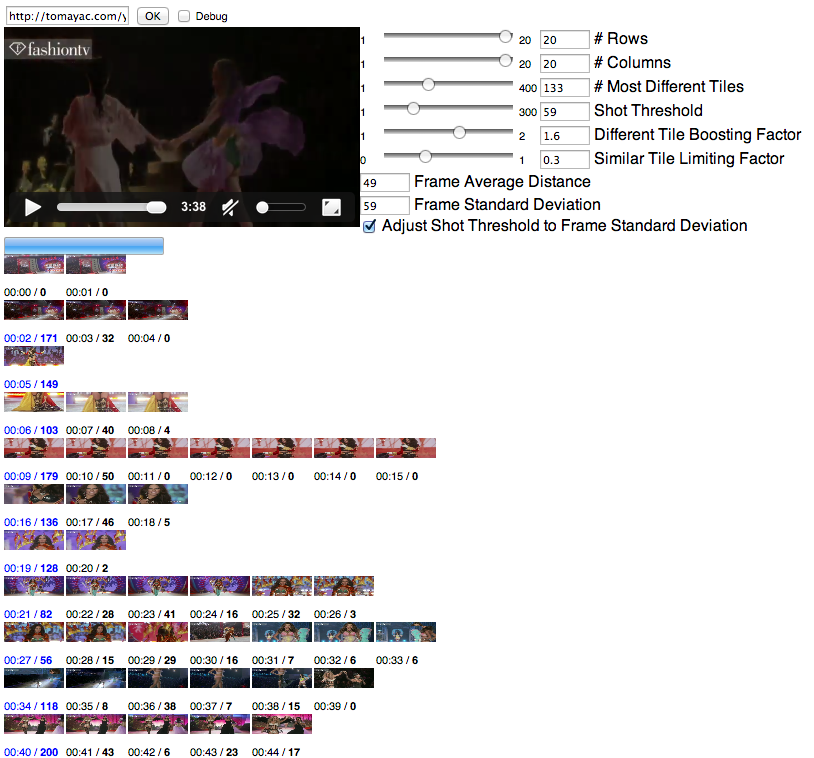
\includegraphics[width=1.0\linewidth]{./vsfashionshowboundaries.png}
  \caption[Excerpt of detected shot boundaries in an event video]
  {Excerpt of detected shot boundaries in a~\emph{Victoria's Secret Fashion Show 2012} event video}
  \label{fig:vsfashionshowboundaries}
\end{figure}

\subsection{Video-contained-in-Video Workflow}

To detect whether a~given video is contained in another,
we follow a~similar approach as outlined in the previous subsection,
with the sole difference being that we need to compare
all detected shot boundary representative photos of the one video
with the ones from the other.
Naturally this approach is even less scalable
with regards to system response time.
The practicable work-around is, as before, to limit oneself
to poster frames delivered by the video hosting platforms.
Our experiments have shown that this approach works very well
for common social network user behavior.
For example, the 3:19 minutes long video of Mark Zuckerberg explaining
the design and engineering challenges behind Facebook's
recently announced Graph Search product was initially published
on Facebook\footnote{\url{https://www.facebook.com/about/graphsearch},
accessed January 22, 2013}, however, people republished the same video 
multiple times on YouTube.
As the YouTube-generated poster frames were similar enough,
and even if the other video meta data like title and description
were different, with the described work-around approach,
we were able to effectively deduplicate the videos.

\section{Conclusion}

In this chapter, we have treated the topic of media item deduplication
from different angles.
We have first defined the meaning of \emph{exact} and \emph{near-duplicate} 
for both photos and videos,
including the special case of a~photo being contained in a~video.
Thereafter, we have introduced an algorithm and application
for video shot boundary detection
whose foundations then served for a~more general
photo deduplication algorithm with semantic features.
We have evaluated the algorithm for two recent events
that had broad social media coverage.
Finally, we have outlined how the photo deduplication algorithm
can be used for basic video deduplication,
albeit minimum system response time requirements
hinder its full applicability in practice.

Media item deduplication of both exact and near-duplicate media items
is a~fundamental step in dealing with huge amounts of social media
and media overload in general.
Highly popular media items not only tend
to retrieve many social interactions on the social network
they were initially shared on, but also tend to get shared
on other social networks.
Derivates of popular media items further add noise
to the social media sharing landscape.
With our media item deduplication algorithms, 
we have effective and efficient tools to deal with social media overload
and to identify the few needles in the cross network haystack. 

\section*{Chapter Notes}
This chapter is partly based on the following publications:
\todo{Add publications}